% !TEX encoding = UTF-8
% !TEX TS-program = pdflatex
% !TEX root = ../tesi.tex

%**************************************************************
\chapter{Contesto aziendale}
\label{cap:introduzione}
%**************************************************************

%**************************************************************
\section{Lab Network}

\begin{figure}[H]
	\begin{center}
	
\includegraphics[scale=0.4]{immagini/LOGO_LABNETWORK.png}
	\caption{Logo \lab{}}
	\end{center}
\end{figure}

\lab{} nasce nel 2016 con lo scopo di aiutare le imprese a creare e ad innovare prodotti e processi attraverso la competenza concreta dei laboratori, sfruttando le potenzialità dei moderni strumenti digitali.\\
L'azienda cerca di collaborare con più partners per poter ottenere una visione maggiore di prodotti e di conseguenza soddisfare i clienti.\\
L'ambiente lavorativo è condiviso con un'altra azienda: \textit{Business Research Srl}, la quale si occupa di soluzioni Software su misura, applicazioni per aziende, E-commerce, Cloud e Hosting.\\
La collaborazione tra Lab Network e Business Research è molto frequente e prevede anche la condivisione del personale.

\section{Organizzazione aziendale}
\lab{} è stata fondata il 24/01/2016 ed è composta da un amministratore unico e una dipendente.
L'organo amministrativo gestisce l'impresa e compie tutte le operazioni necessarie per il raggiungimento dell'oggetto sociale.
Le attività principali esercitate dallo staff sono:
\begin{itemize}
\item ideazione e gestione di sistemi informatici per la condivisione di conoscenze sulle nuove tecnologie;
\item noleggio di macchine e attrezzature per ufficio;
\item commercio all'ingrosso di hardware e software;
\item noleggio di kit di formazione e materiale didattico innovativo (stampanti 3D, schede elettroniche, ecc..);
\item organizzazione e promozione di corsi di formazione per aziende e disoccupati;
\item partecipazione a fiere ed eventi di settore;
\item consulenza in ambito tecnologico e innovativo.
\end{itemize}
\subsection{Metodologia di lavoro e processi aziendali}
Lo schema che l'azienda ha sviluppato si divide in tre fasi:
\begin{itemize}
\item Creare l’interesse attraverso politiche di marketing discutendo di temi specifici ad alto impatto mediatico;
\item Raccogliere gruppi omogenei che condividono l'interesse ad una specifica tecnologia;
\item Attraverso attività di consulenza e formazione si cerca da un lato di capire le esigenze produttive e dall’altro le potenzialità che una digitalizzazione (hardware o software) può contribuire alla crescita di una PMI.
\end{itemize}

\subsection{La metodologia agile}
\begin{figure}[H]
	\begin{center}
	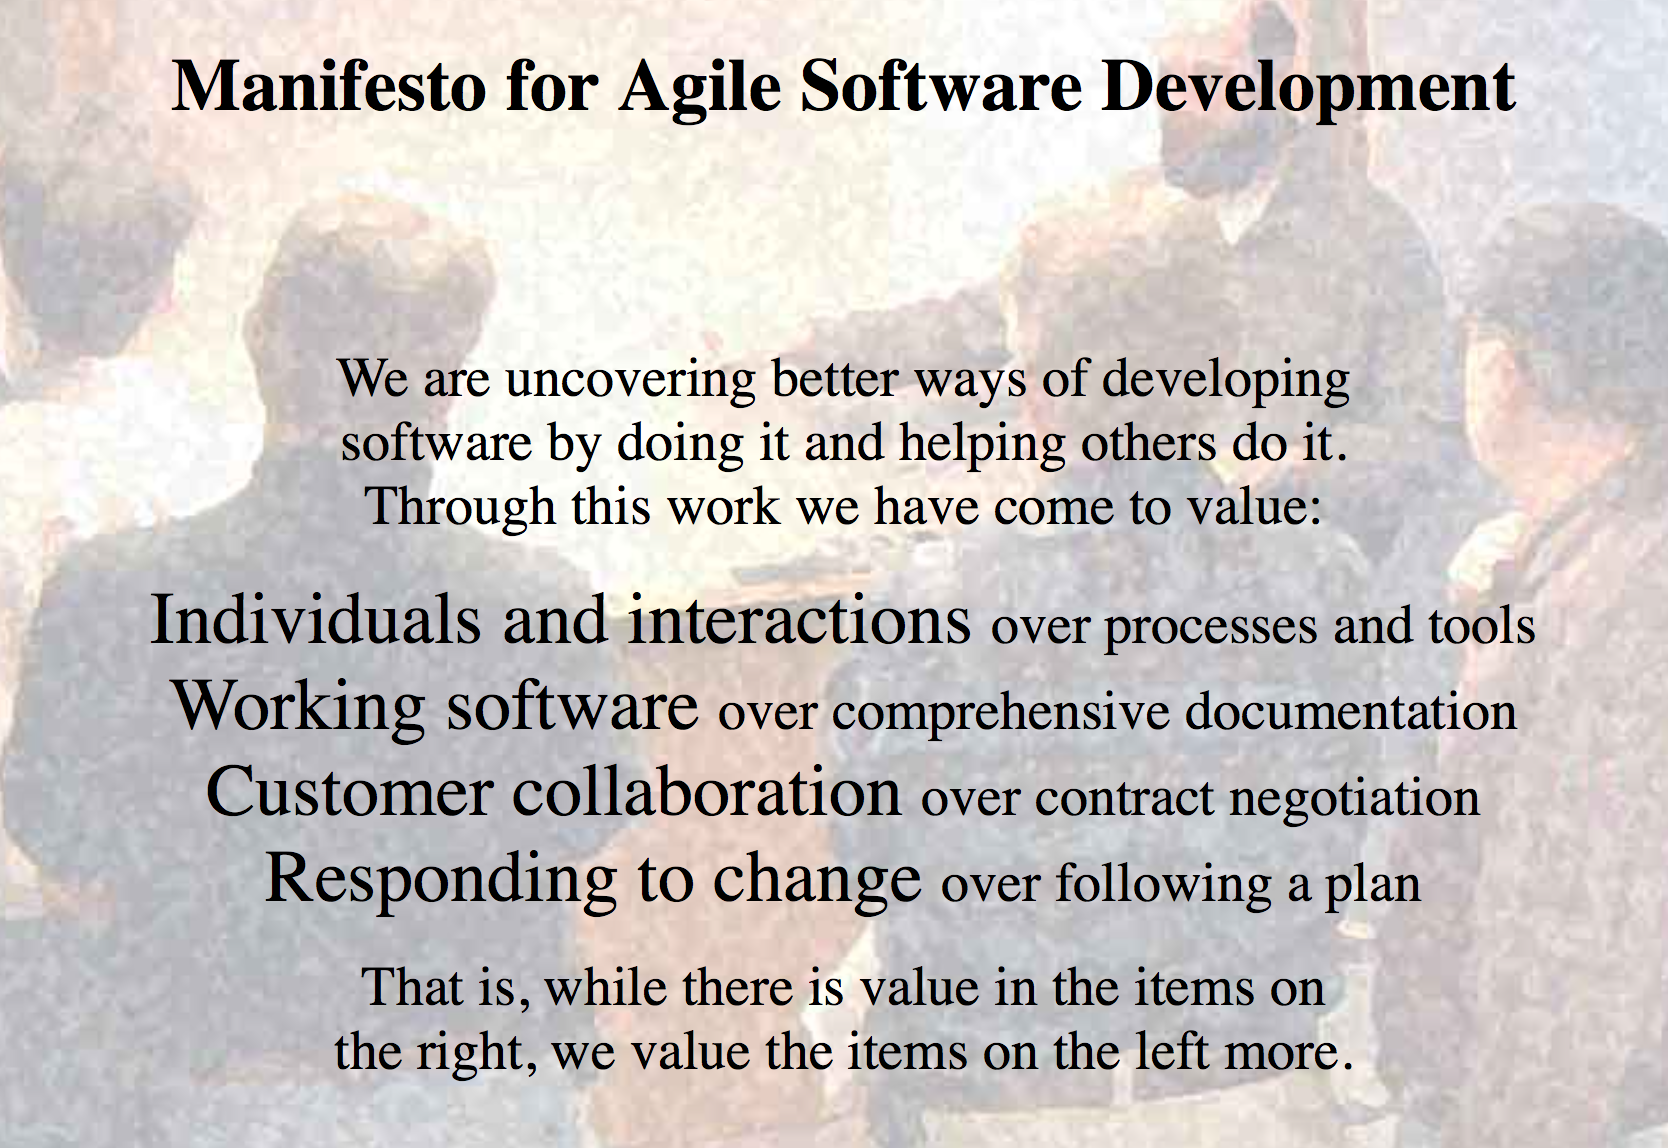
\includegraphics[scale=0.25]{immagini/agile_manifesto.png}
	\caption{I principi del manifesto agile}
	\small{\textbf{Fonte:} \url{http://agilemanifesto.org}}
	\end{center}
\end{figure}
\lab{} segue i principi della metodologia agile durante i processi di sviluppo di un nuovo progetto.
\begin{enumerate}

\item \textbf{Gli individui e le interazioni più che i processi e gli strumenti.}\\
\\
\tab \lab{} infatti ha un approccio per lo sviluppo di un progetto molto legato alla comunicazione col cliente. Il metodo di lavoro dell'azienda e i processi ad esso legati sono flessibili e si adattano alle richieste.

\item \textbf{Il software funzionante più che la documentazione esaustiva.}\\
\\
La priorità è sempre sul software. Vengono sviluppati molti prototipi da esporre al cliente affinando via via in modo incrementale la soluzione definitiva. Questo approccio consente di far accrescere la soddisfazione del cliente.

\item \textbf{La collaborazione col cliente più che la negoziazione dei contratti.}\\
\\
Secondo \lab{} il cliente è parte integrante del progetto infatti esso viene costantemente aggiornato sullo stato durante tutta la fase di sviluppo e interrogato sul suo stato di soddisfazione. Una buona collaborazione è un punto fondamentale per il successo del progetto.

\item \textbf{Rispondere al cambiamento più che seguire un piano.}\\
\\
La pianificazione iniziale passa in secondo piano dal momento in cui si presenta la necessità di cambiare, nel caso di richieste da parte del cliente, adozione di tecnologie differenti ecc.

\end{enumerate}

\subsection{Tecnologie}

\subsubsection{Elettronica e Hardware}
A supporto dei processi di prototipazione, \lab{} utilizza diverse piattaforme hardware come ad esempio \textit{Arduino}, \textit{Raspberry Pi}, \textit{Intel UP Square}, \textit{Asus TinkerBoard} ecc.\\
\lab{}, inoltre, sfrutta le potenzialità della stampa 3D e del disegno CAD per creare modelli prototipali in modo rapido. La disponibilità in azienda di 3 stampanti 3D permette di ridurre il tempo per la realizzazione dei prototipi da proporre al cliente.

\begin{figure}[H]
	\begin{center}
	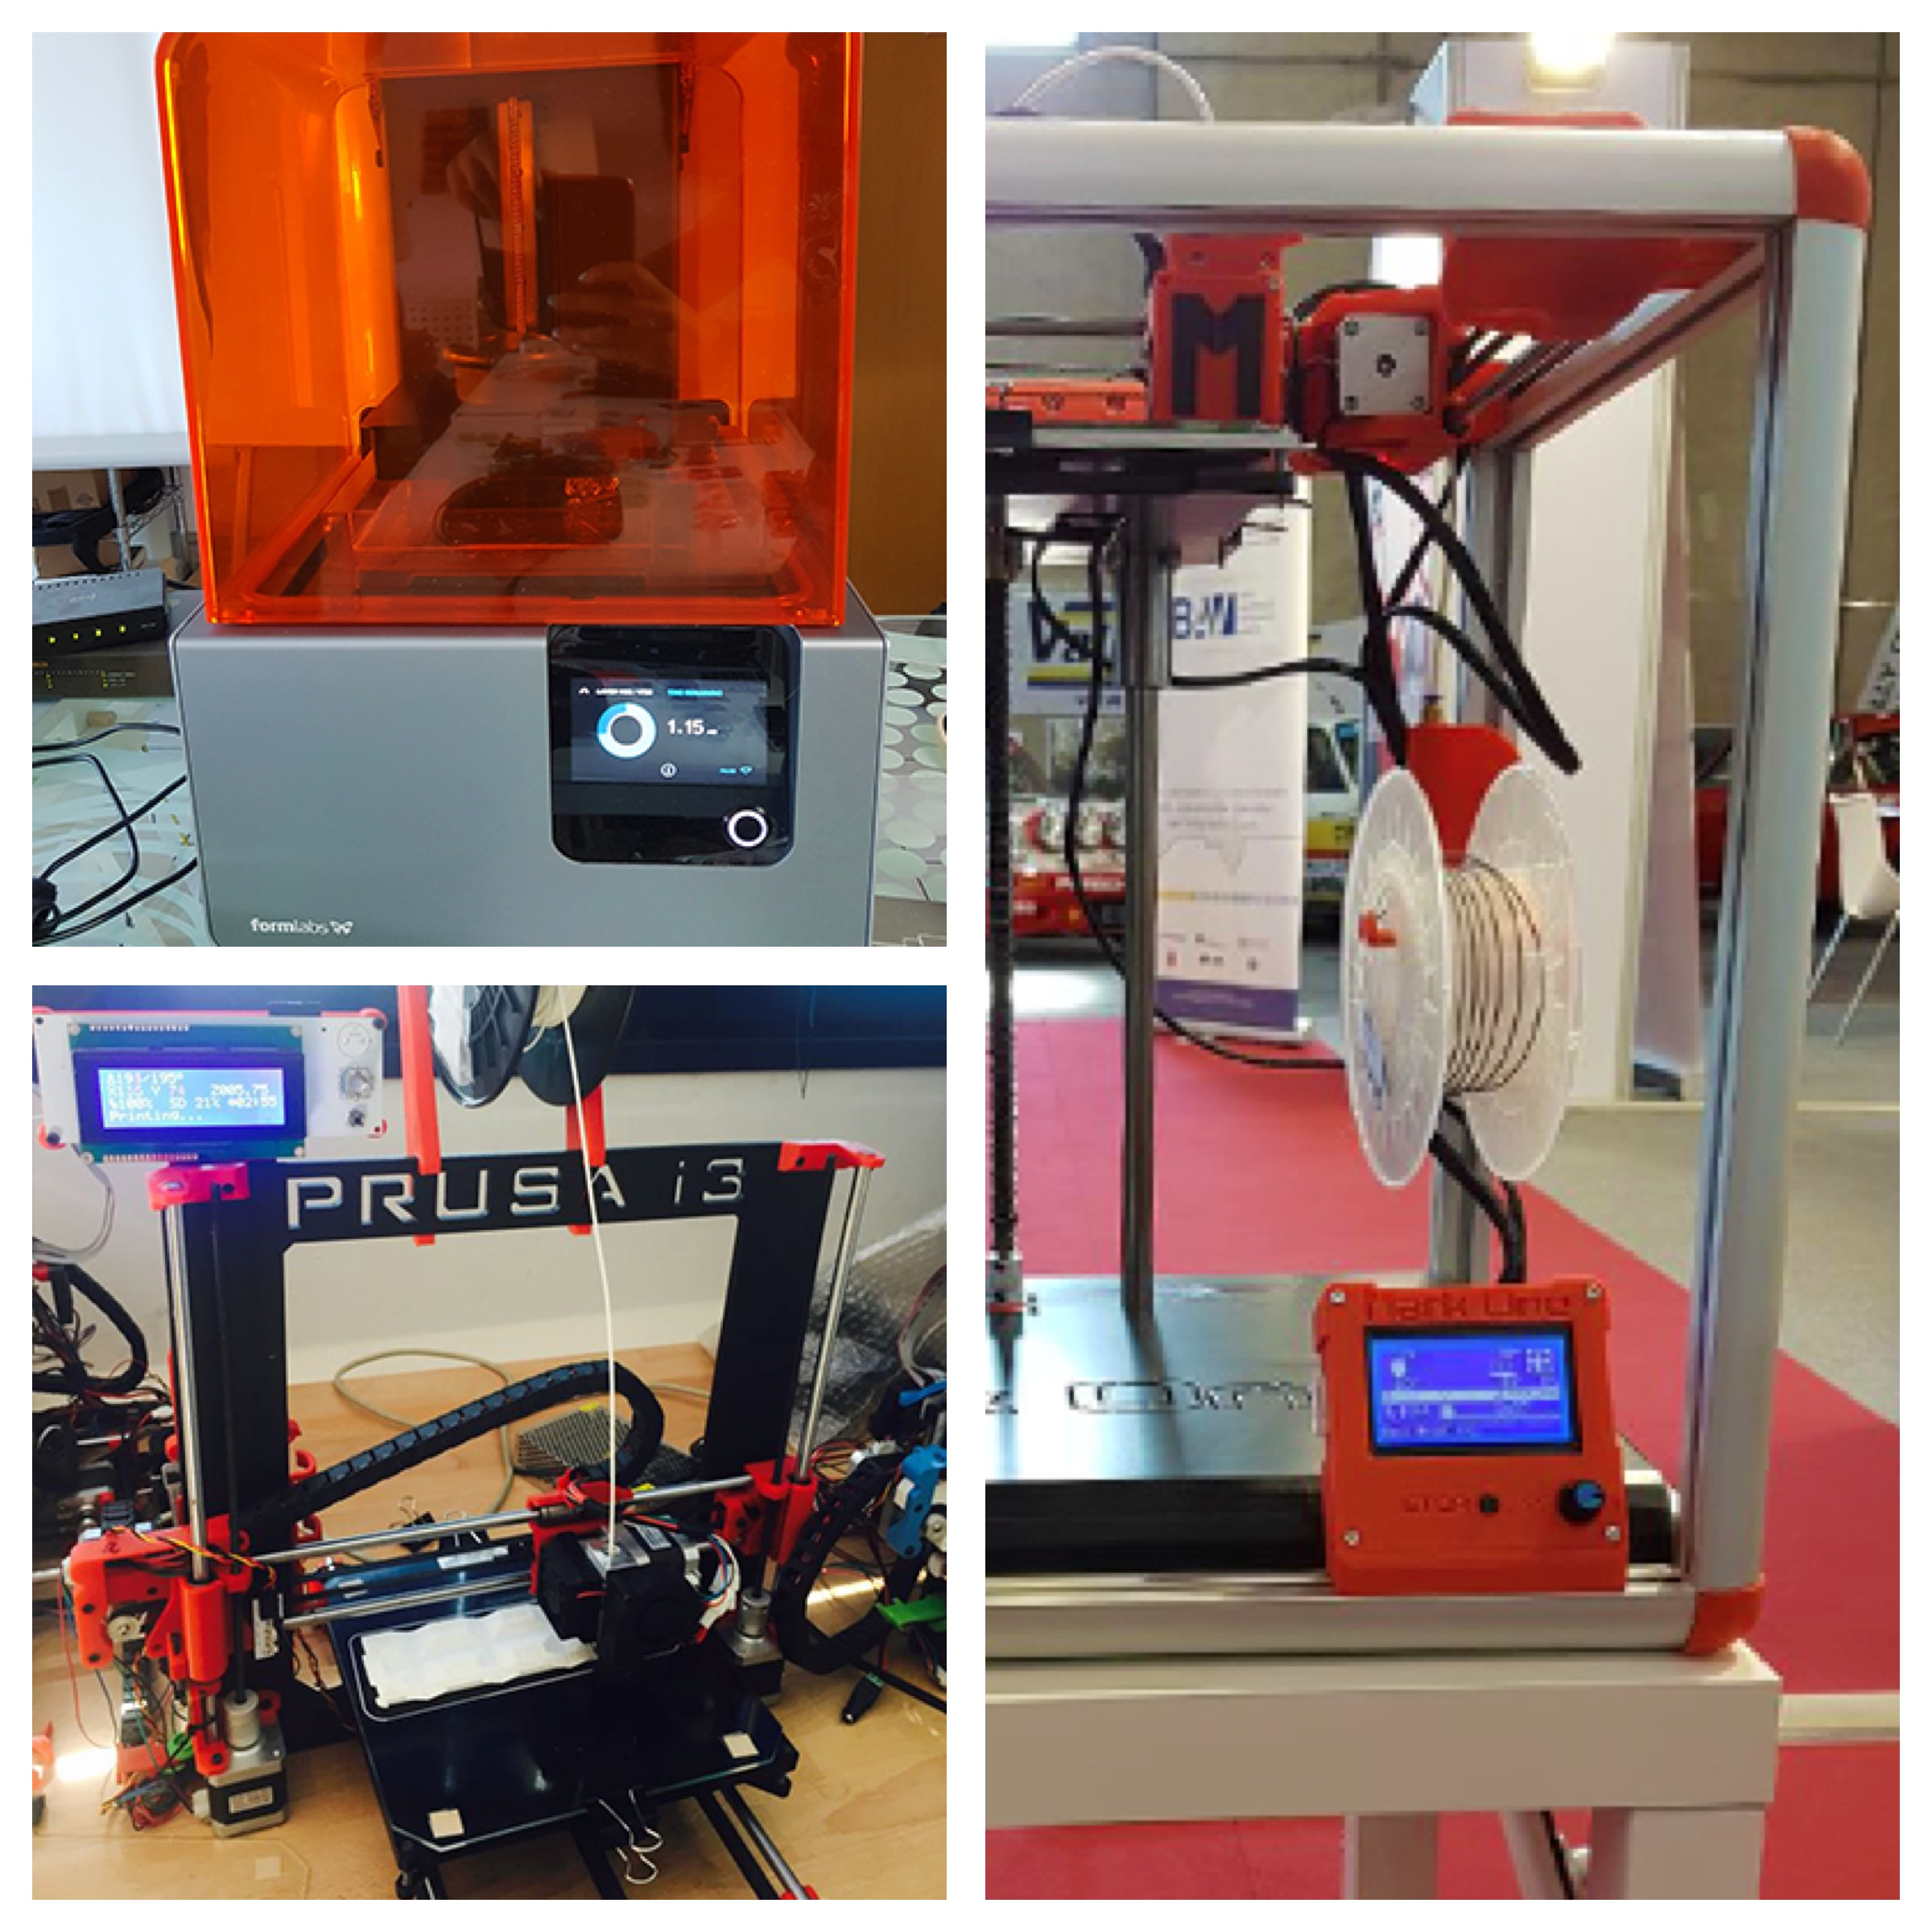
\includegraphics[scale=0.07]{immagini/stampanti.jpg}
	\caption{Le stampanti 3D in dotazione a \lab{}}
	\end{center}
\end{figure}

\subsubsection{Realtà virtuale e aumentata}
L'azienda utilizza software e strumenti per lo studio e lo sviluppo in ambito della realtà virtuale ed aumentata.
Nel dettaglio, è stato utilizzato il motore grafico \textit{Unreal Engine} per lo sviluppo dell'ambiente virtuale relativo al Vitruvian Game: per utilizzare e testare tale ambiente, \lab{} utilizza il visore \textit{Vive} prodotto da \textit{HTC}.\\
L'azienda, in ambito di realtà aumentata, utilizza la piattaforma \textit{Unity} per lo sviluppo di nuove applicazioni.\\

\subsubsection{Tecnologie di supporto}
A supporto dei processi di sviluppo, l'azienda utilizza la piattaforma web di \textit{GitLab}, che consente la gestione di repository Git e di funzioni trouble ticket.\\
L'utilizzo di questa piattaforma permette il controllo della configurazione e del versionamento di un software, oltre che la gestione di ticket.

\begin{figure}[H]
	\begin{center}
	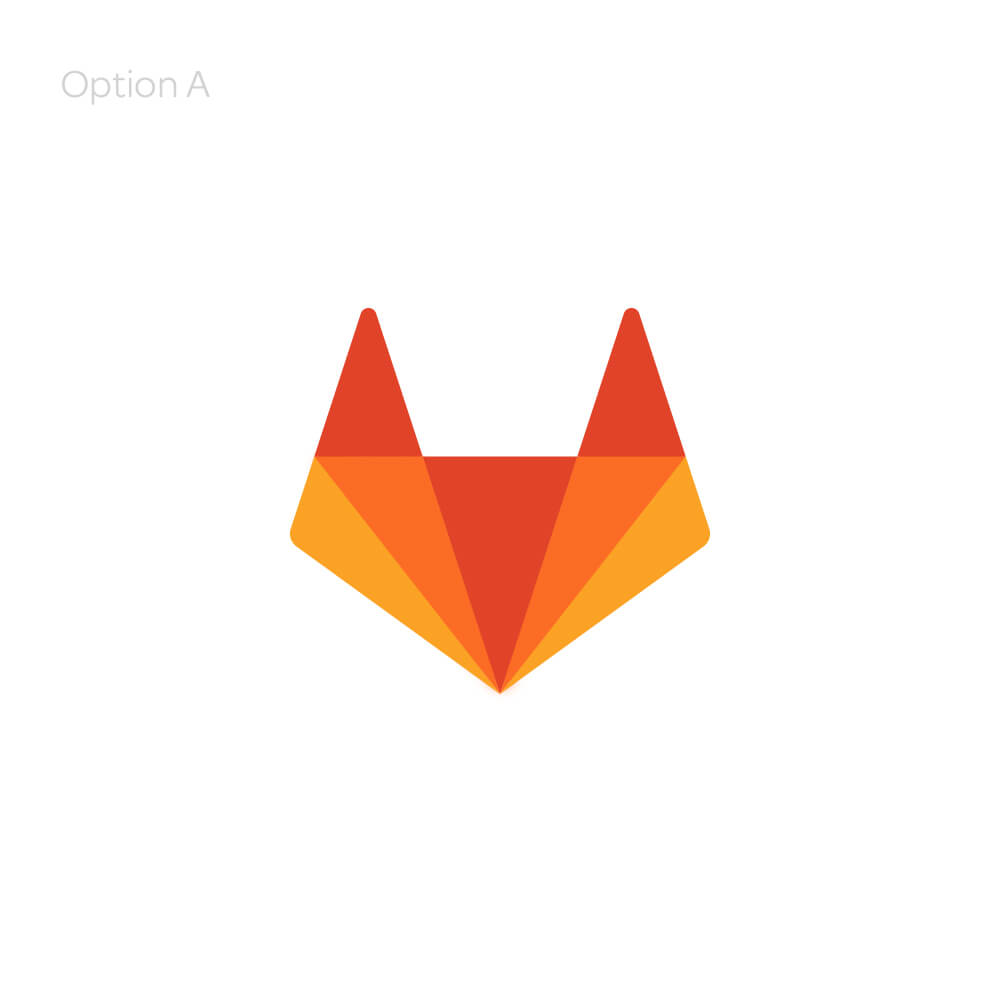
\includegraphics[scale=0.15]{immagini/gitlab.jpg}
	\caption{Logo GitLab}
	\small{\textbf{Fonte:} \url{https://about.gitlab.com/2015/05/18/a-new-gitlab-logo/}}
	\end{center}
\end{figure}

\subsubsection{Applicazioni mobile}
Per lo svilupppo di applicazioni mobile, sia Android che iOS, \lab{} utlizza gli ambienti di sviluppo \textit{Android Studio} e \textit{Xcode}.
\\I linguaggi di programmazione utilizzati sono:
\begin{itemize}
\item Android Studio
	\begin{itemize}
		\item Java
	\end{itemize}
\item Xcode
	\begin{itemize}
		\item C++
		\item C
		\item Swift
		\item Objective-C
	\end{itemize}
\end{itemize}

\begin{figure}[H]
\centering

\includegraphics[scale=0.15]{immagini/android_studio.png}\quad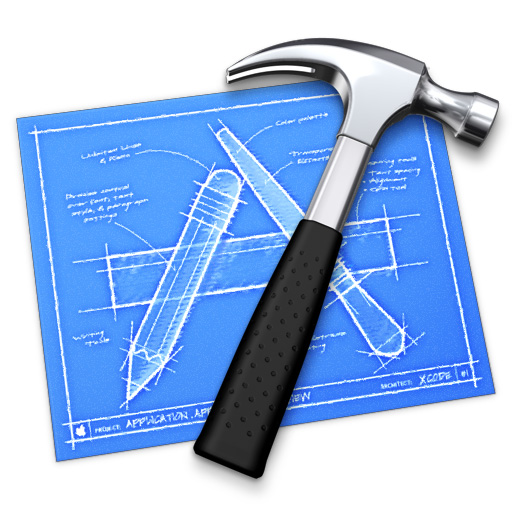
\includegraphics[scale=0.15]{immagini/xcode.jpg}
\caption{Loghi a partire da sinistra: Android Studio e Xcode}
\small{\textbf{Fonte (Android Studio):} \url{https://developer.android.com/studio/}}\\
\small{\textbf{Fonte (Xcode):} \url{https://developer.apple.com/xcode/}}
\end{figure}

\subsubsection{Deep Learning e intelligenza artificiale}
Utilizzando Intel Movidius, \lab{} sta attualmente sviluppando un progetto che consiste nella previsione di futuri incidenti e infortuni sul lavoro.\\
Sfruttando le tecniche di \textit{deep learnign} messe a disposizione dall'hardware, si è in grado, analizzando grandi dati riguardanti incidenti passati, di effettuare una stima sui possibili incidenti futuri.

\section{Prodotti e servizi}
\subsection{Prodotti}
\textbf{VITRUVIAN GAME – Wingsuit VR}
\\
Dalla collaborazione con Intel\textsuperscript{\textregistered} nasce il simulatore di volo con tuta alare ispirato al capolavoro di Leonardo.\\
Il progetto prevede l'utilizzo del visore HTC Vive affiancato ad uno scenario virtuale sviluppato con motore grafico \textit{Unreal Engine}. Per i movimenti sugli assi sono stati impiegati dei motori per automazione industriale.
\\
\begin{figure}[H]
	\begin{center}
	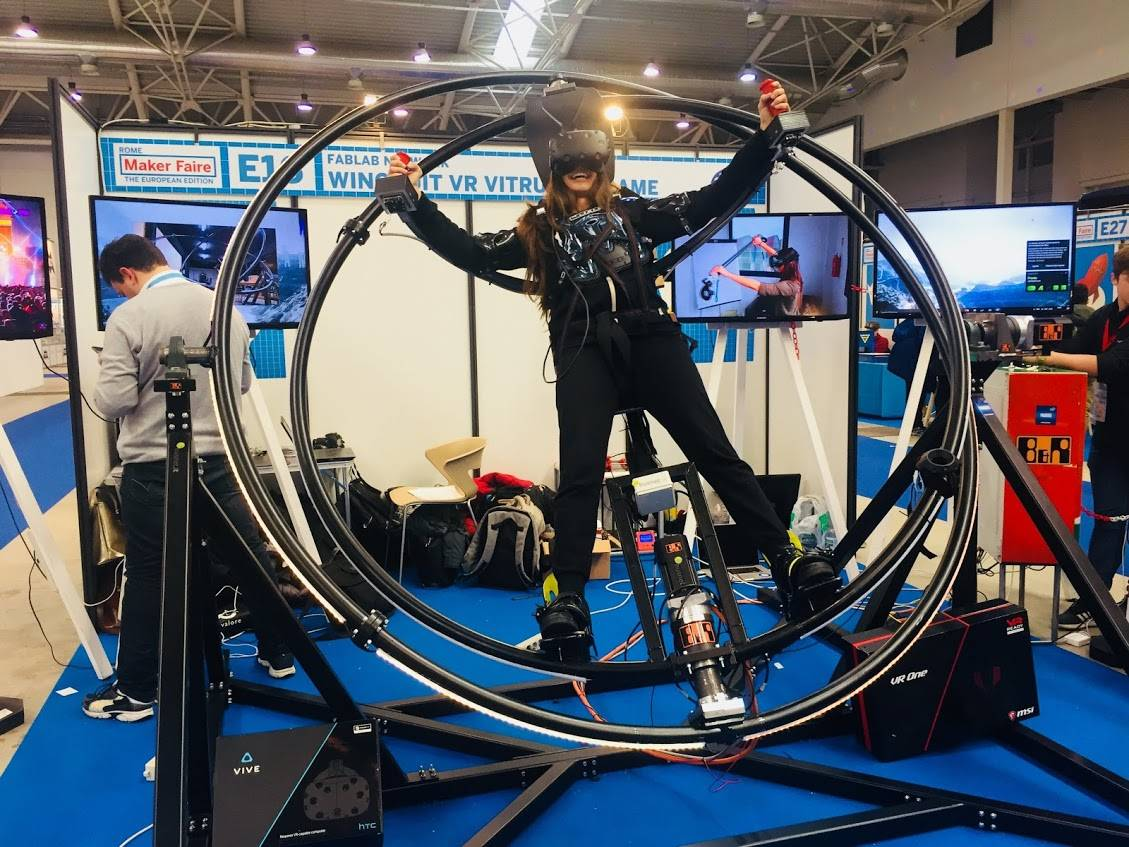
\includegraphics[scale=0.15]{immagini/vitruvian.jpg}
	\caption{Vitruvian Game - Il simulatore di volo con tuta alare}
	\end{center}
\end{figure}

\noindent \textbf{FabKey}
\\
La serratura smart connessa ad internet permette l'apertura di una porta controllando una lista di accessi presente in cloud. Funziona tramite tag \gls{NFC} o barcode. Il prodotto è rivolto principalmente ai \gls{FabLab}, ma si adatta facilmente a qualsiasi contesto in cui sia richiesto il controllo degli accessi.
\\
\\
\textbf{Smart Meter}
\\
Un metro 4.0 capace di misurare superfici complesse e inviare direttamente i dati al software gestionale, in aggiunta anche il monitoraggio in tempo reale di quando, dove e per quanto tempo è stato utilizzato dal singolo addetto.

\subsection{Servizi}
I servizi che \lab{} offre ai propri clienti sono:
\begin{itemize}
\item \textbf{Progettazione:} corsi di formazione su misura, \gls{counseling} e \gls{workshop} per imparare a sfruttare in modo professionale: 3D Printing, schede elettroniche, \gls{cz}, realtà virtuale e aumentata, sviluppo App, prototipazione, \gls{bigd}, \gls{iot} ecc.
\item \textbf{Noleggio:} Kit e attrezzature come stampanti 3D, schede elettroniche (\gls{arduino}, \gls{rpi}, Intel) visori VR, pc e notebook, videoproiettori; affitto aule didattiche per \gls{makers} e industria 4.0.
\item \textbf{Personale qualificato:} per i clienti sono a disposizione docenti, tecnici di laboratorio e consulenti specializzati nei principali ambiti di innovazione digitale.
\item \textbf{Assistenza:} pianificazione e costruzione su misura di progetti innovativi sviluppando idee imprenditoriali.
\end{itemize}

\section{Lab Network e innovazione}
\lab{} si è sviluppata nell’ambito della \textit{smart specialisation} attraverso logiche di coinvolgimento di una comunità di utenti misti che provengono prevalentemente dal mondo aziendale e accademico. 
L'azienda si propone come punto di riferimento per l’innovazione \textit{Open Source} nel territorio del Veneto, tramite la rete interconnessa dei \gls{FabLab} esistenti, e promuovendosi come centro privilegiato di interscambio di conoscenza.\\
Comprendendo che il tessuto imprenditoriale veneto è composto quasi totalmente di piccole e medie imprese dinamiche ed interconnesse, con un’industrializzazione diffusa ed una forte vocazione di tipo manifatturiero, \lab{} si è posta l’obiettivo di contribuire, attraverso strumenti e modalità di funzionamento specifici, a sviluppare ed attuare la strategia Regionale della ``Fabbrica Intelligente Del Futuro''.\\
Questa mira ad indirizzare la trasformazione del settore manifatturiero verso nuovi prodotti, processi e tecnologie, attraverso lo sviluppo di attività di ricerca di alto livello.

\subsection{Smart Specialisation Strategy}
\begin{figure}[H]
	\begin{center}
	
\includegraphics[scale=0.4]{immagini/join-s3p.png}
	\caption{Logo della piattaforma della Smart Specialisation.}
	\small{\textbf{Fonte:} \url{http://s3platform.jrc.ec.europa.eu}}
	\end{center}
\end{figure}

La \textit{Smart Specialisation} è una strategia concepita nell'ambito della politica di coesione riformata dalla Commissione Europea.\\
La specializzazione intelligente è un approccio fondato sull'individuazione di aree strategiche di intervento, basate sia sull'analisi dei punti di forza e del potenziale dell'economia sia su un processo di scoperta imprenditoriale con ampio coinvolgimento delle parti interessate.\\
Abbraccia un'ampia visione dell'innovazione, inclusi, ma certamente non limitati a, approcci incentrati sulla tecnologia e supportati da efficaci meccanismi di monitoraggio.\\
\\
Attraverso il portale dedicato che \lab{} utilizza per scambiare informazioni, le aziende e i makers possono lavorare in autonomia, ma condividendo le informazioni che possono essere attinte per le attività che competono a più soggetti.\\
\\
L'\gls{SWOT} sulla realtà delle PMI venete, contenuta nella Smart Specialisation Strategy, evidenzia come ci sia uno scarso utilizzo di tecnologie ICT, scarsa disponibilità di laboratori di proprietà, bassi investimenti in ricerca, difficoltà a sciluppare progetti innovativi e ridotta capacità di reperire risorse e professionalità necessarie. 
L'obiettivo di \lab{} è quello di colmare queste lacune mettendo a disposizione alle azienda un'area di lavoro a costi contenuti dove poter utilizzare i principali strumenti di innovazione digitale come: stampanti 3D, kit elettronici, macchine a controllo numerico, frese digitali e taglio laser. Tutto quest può essere definito come un laboratorio per studiare la fase prototipale.
\\
In pratica \lab{} vuole contribuire a portare l'innovazione e la tecnologia all'interno delle PMI che ancora non si sono interfacciate a questo ''nuovo mondo``.

